\documentclass[paper=a4, fontsize=11pt]{scrartcl} % A4 paper and 11pt font size

% ---- Entrada y salida de texto -----

\usepackage[T1]{fontenc} % Use 8-bit encoding that has 256 glyphs
\usepackage[utf8]{inputenc}
\usepackage[a4paper, total={6in, 9in}]{geometry}
%\usepackage{fourier} % Use the Adobe Utopia font for the document - comment this line to return to the LaTeX default

% ---- Idioma --------

\usepackage[spanish, es-tabla]{babel} % Selecciona el español para palabras introducidas automáticamente, p.ej. "septiembre" en la fecha y especifica que se use la palabra Tabla en vez de Cuadro

% ---- Otros paquetes ----


\usepackage{amsmath,amsfonts,amsthm} % Math packages
%\usepackage{graphics,graphicx, floatrow} %para incluir imágenes y notas en las imágenes
\usepackage{graphics,graphicx, float, url} %para incluir imágenes y colocarlas
\usepackage{eurosym}
% Para hacer tablas comlejas
%\usepackage{multirow}
%\usepackage{threeparttable}

%\usepackage{sectsty} % Allows customizing section commands
%\allsectionsfont{\centering \normalfont\scshape} % Make all sections centered, the default font and small caps

%Esto es para hipervinculos
\usepackage[hidelinks]{hyperref}

%list code
\usepackage{listings}



\usepackage{tikz}
\usetikzlibrary{positioning}
% para grafos


\hypersetup{
    colorlinks=true,
    linkcolor=blue,
    filecolor=blue,      
    urlcolor=blue,
    citecolor=blue,
    pdftitle={Overleaf Example},
    pdfpagemode=FullScreen,
    }

\urlstyle{same}
\usepackage{gensymb}
\usepackage{fancyhdr} % Custom headers and footers
\pagestyle{fancyplain} % Makes all pages in the document conform to the custom headers and footers
\fancyhead{} % No page header - if you want one, create it in the same way as the footers below
\fancyfoot[L]{} % Empty left footer
\fancyfoot[C]{} % Empty center footer
\fancyfoot[R]{\thepage} % Page numbering for right footer
\renewcommand{\headrulewidth}{0pt} % Remove header underlines
\renewcommand{\footrulewidth}{0pt} % Remove footer underlines
\setlength{\headheight}{13.6pt} % Customize the height of the header

\numberwithin{equation}{section} % Number equations within sections (i.e. 1.1, 1.2, 2.1, 2.2 instead of 1, 2, 3, 4)
\numberwithin{figure}{section} % Number figures within sections (i.e. 1.1, 1.2, 2.1, 2.2 instead of 1, 2, 3, 4)
\numberwithin{table}{section} % Number tables within sections (i.e. 1.1, 1.2, 2.1, 2.2 instead of 1, 2, 3, 4)

\setlength\parindent{0pt} % Removes all indentation from paragraphs - comment this line for an assignment with lots of text

\newcommand{\horrule}[1]{\rule{\linewidth}{#1}} % Create horizontal rule command with 1 argument of height
\usepackage{subcaption}

\title{	
\normalfont \normalsize 
\textsc{{\textbf{Aprendizaje Profundo (2024-2025)}} \\ Máster en Robótica e Inteligencia Artificial \\ Universidad de León} \\ [20pt] % Your university, school and/or department name(s)
\horrule{0.5pt} \\[0.4cm] % Thin top horizontal rule
\huge Práctica 4 \\   % The assignment title
\horrule{1.5pt} \\[0.2cm] % Thick bottom horizontal rule
}

\author{Sheila Martínez Gómez\\
Alejandro Mayorga Caro\\
Ángel Morales Romero\\
}
 % Nombre y apellidos
 % Incluye la fecha actual

\begin{document}

\maketitle
\newpage %inserta un salto de página

\tableofcontents % para generar el índice de contenidos
\pagebreak
\section{Abstract}

En esta práctica se implementan y comparan diferentes técnicas de reducción de dimensionalidad y clasificación utilizando un conjunto de datos sintético en \(\mathbb{R}^{10}\). El objetivo es evaluar el rendimiento de las siguientes técnicas:

\begin{itemize}
    \item Sammon Mapping
    \item PCA (Principal Component Analysis)
    \item LDA (Linear Discriminant Analysis)
    \item t-SNE (t-distributed Stochastic Neighbor Embedding)
    \item Redes Neuronales Encoder-Decoder
\end{itemize}

Además, se analiza el rendimiento de un clasificador basado en un Encoder-Decoder, congelando el modelo.

\section{Generación del Dataset}

El conjunto de datos consta de 3 grupos o esferas generadas aleatoriamente en un espacio de 2 dimensiones (\(\mathbb{R}^{2}\)), y giradas en un espacio de 10 dimensiones (\(\mathbb{R}^{10}\)). Las clases se etiquetarán como Clase 0, Clase 1 y Clase 2. Este conjunto fue generado con el siguiente código:

\begin{verbatim}
def generate_spheres(samples_per_class, dim=10):
    np.random.seed(0)
    centers = [np.zeros((1, dim)), np.ones((1, dim)) * 2, np.ones((1, dim)) * 4]
    data, labels = [], []
    for idx, center in enumerate(centers):
        sphere = np.random.normal(size=(samples_per_class, dim)) + center
        data.append(sphere)
        labels.extend([idx] * samples_per_class)
    return np.vstack(data), np.array(labels)
\end{verbatim}

El conjunto generado tiene un total de 600 muestras, distribuidas equitativamente entre las tres clases.

\begin{figure}[H]
\centering
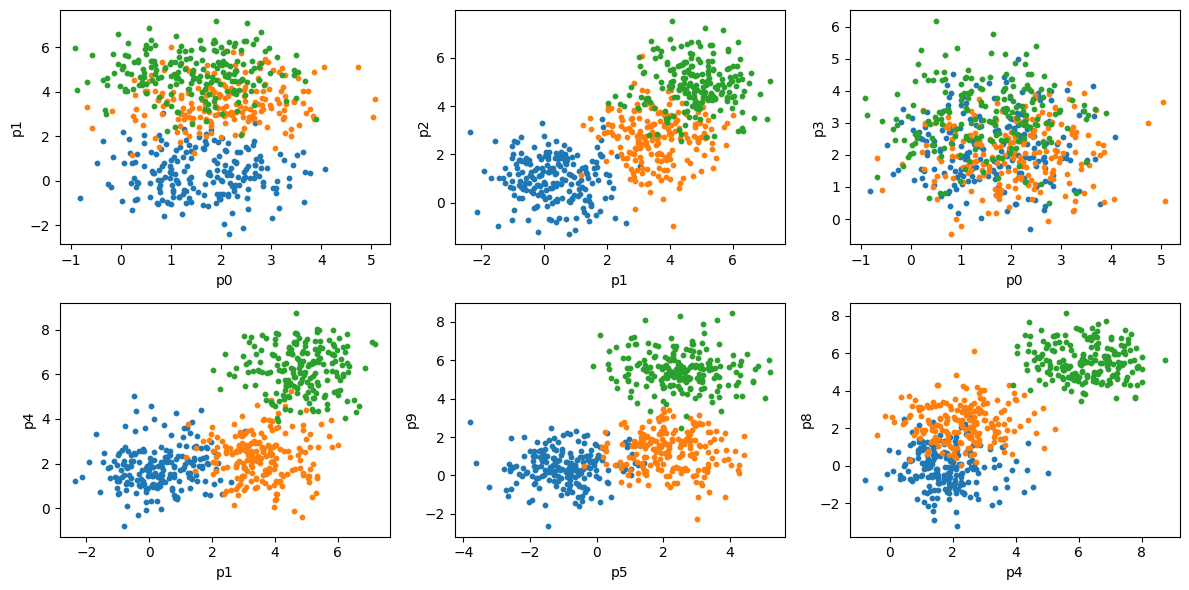
\includegraphics[width=0.8\textwidth]{images/dataset_projection.png}
\caption{Proyección del conjunto de datos original en diferentes dimensiones.}
\end{figure}

\section{Métodos de Reducción de Dimensionalidad}

En esta sección se muestran los diferentes métodos de reducción de dimensionalidad que se han utilizado, con el objetivo de simplificar los datos, mejorar el rendimiento del modelo a aplicar y simplificar la visualización del \textit{dataset}.

Los métodos aplicados para reducir las dimensiones de los datos son los siguientes:

\subsection{Sammon Mapping}
El Sammon Mapping es un método no lineal que minimiza las distorsiones en las distancias entre puntos al proyectarlos a un espacio de menor dimensión. La implementación utiliza la biblioteca de `sklearn`:

\begin{verbatim}
from sklearn.manifold import MDS

sammon = MDS(n_components=2, metric=True)
X_sammon = sammon.fit_transform(X)
\end{verbatim}

\begin{figure}[H]
\centering
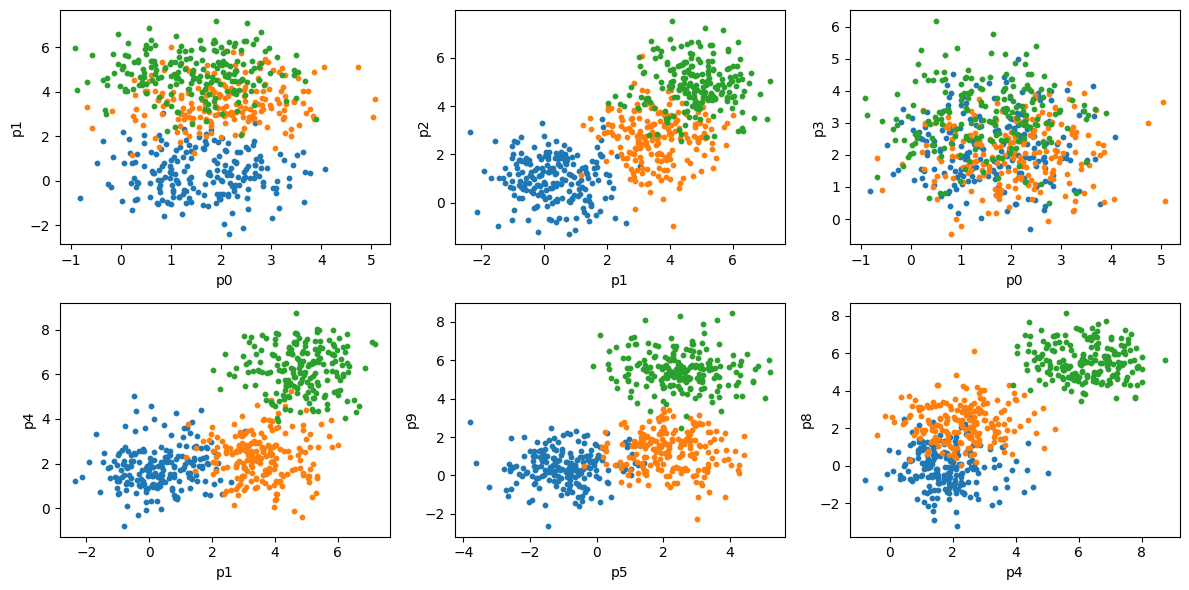
\includegraphics[width=0.8\textwidth]{images/sammon_projection.png}
\caption{Proyección de los datos en 2D usando Sammon Mapping.}
\end{figure}

\subsection{PCA}
El análisis de componentes principales busca las direcciones de máxima varianza en los datos. En este caso, se seleccionaron las dos primeras componentes principales:

\begin{verbatim}
from sklearn.decomposition import PCA

pca = PCA(n_components=2)
X_pca = pca.fit_transform(X)
\end{verbatim}

\begin{figure}[H]
\centering
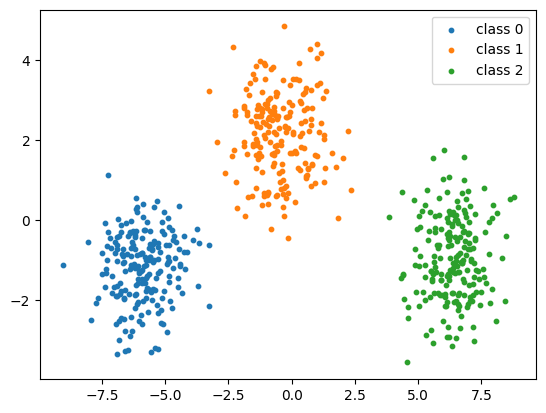
\includegraphics[width=0.8\textwidth]{images/pca_projection.png}
\caption{Proyección de los datos en 2D usando PCA.}
\end{figure}

\subsection{LDA}
El análisis discriminante lineal maximiza la separación entre clases al proyectar los datos a un espacio de menor dimensión:

\begin{verbatim}
from sklearn.discriminant_analysis import LinearDiscriminantAnalysis as LDA

lda = LDA(n_components=2)
X_lda = lda.fit_transform(X, y)
\end{verbatim}

\begin{figure}[H]
\centering
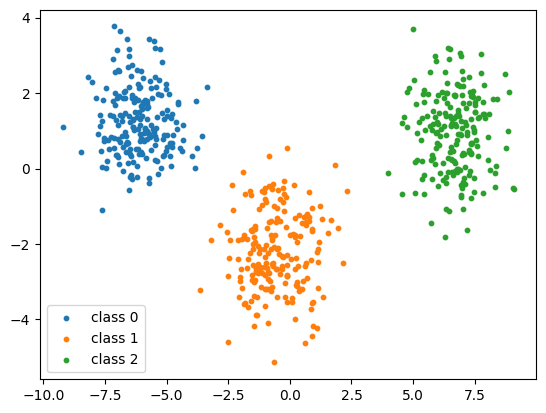
\includegraphics[width=0.8\textwidth]{images/lda_projection.png}
\caption{Proyección de los datos en 2D usando LDA.}
\end{figure}

\subsection{t-SNE}
El t-SNE (\textit{t-Distributed Stochastic Neighbor Embedding})  preserva las relaciones locales en los datos, útil para visualización en 2D ya que permite la división gráfica de conjuntos difícilmente separables mediante fronteras lineales. Es importante señalar que este método tiene una componente estocástica, que controlaremos mediante la selección de un \textit{random\_state} para permitir la replicabilidad.

\begin{verbatim}
from sklearn.manifold import TSNE

tsne = TSNE(n_components=2, random_state=42)
X_tsne = tsne.fit_transform(X)
\end{verbatim}

\begin{figure}[H]
\centering
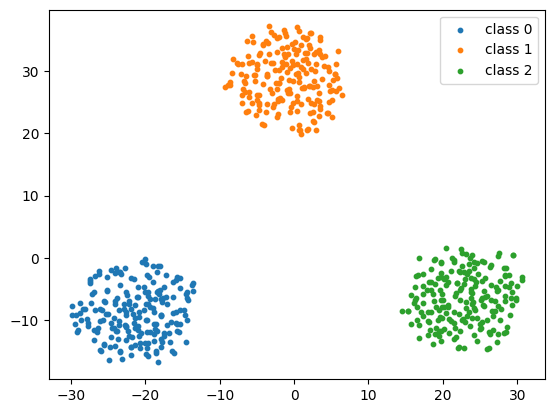
\includegraphics[width=0.8\textwidth]{images/tsne_projection.png}
\caption{Proyección de los datos en 2D usando t-SNE.}
\end{figure}

\section{Red Neuronal Encoder-Decoder}

Se utilizó una red neuronal Encoder-Decoder para aprender una representación comprimida de los datos. El modelo fue definido como:

\begin{verbatim}
def build_encoder_decoder(input_dim=10, encoded_dim=2):
    input_layer = layers.Input(shape=(input_dim,), name='Input')
    
    # Encoder
    encoded = layers.Dense(8, activation='relu', name='Dense8_encoder')(input_layer)
    encoded = layers.Dense(6, activation='relu', name='Dense6_encoder')(encoded)
    encoded = layers.Dense(4, activation='relu', name='Dense4_encoder')(encoded)
    encoded = layers.Dense(encoded_dim, activation='linear', name=f'Dense{encoded_dim}')
                                                                               (encoded)

    # Decoder
    decoded = layers.Dense(4, activation='relu', name='Dense4_decoder')(encoded)
    decoded = layers.Dense(6, activation='relu', name='Dense6_decoder')(decoded)
    decoded = layers.Dense(8, activation='relu', name='Dense8_decoder')(decoded)
    decoded = layers.Dense(input_dim, activation='linear', name='Output')(decoded)
    
    # Modelo completo
    autoencoder = models.Model(input_layer, decoded, name='Autoencoder')
    
    # Encoder separado para reutilización
    encoder = models.Model(input_layer, encoded, name='Encoder')

    return autoencoder, encoder

\end{verbatim}

Posteriormente se dividirán los datos en tres conjuntos (entrenamiento, validación y test). 

\begin{verbatim}
    xtrn, xtst, ytrn, ytst = train_test_split(X, y, test_size=0.2,
                                              stratify=y, random_state=42)
    xtrn, xval, ytrn, yval = train_test_split(xtrn, ytrn, test_size=0.1,
                                              stratify=ytrn, random_state=42)

\end{verbatim}

Este modelo fue entrenado durante 150 épocas, con un valor de \textit{batch\_size} de \lstinline{xtrn.shape[0]//4} y utilizando \textit{Early-stopping}.

Esto otorga unos resultados positivos en pérdidas, como se puede ver en la siguiente gráfica:

\begin{figure}[H]
\centering
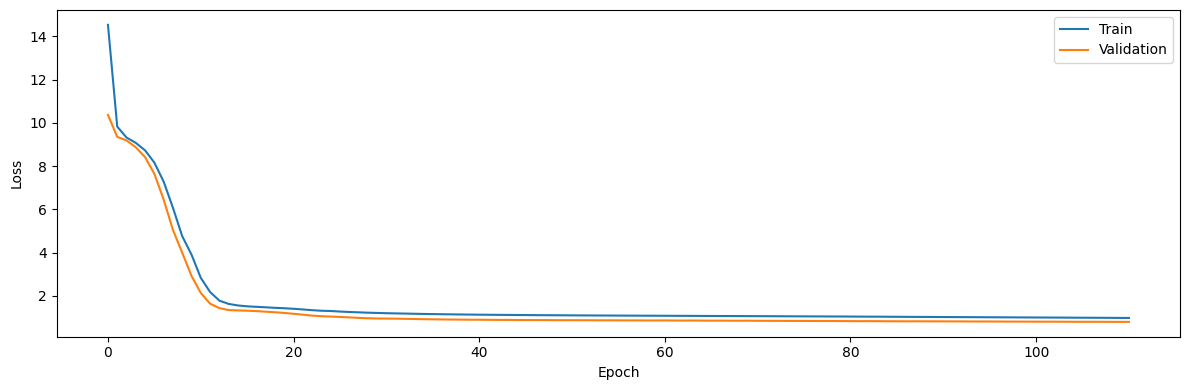
\includegraphics[width=0.8\textwidth]{images/loss_encoder.png}
\caption{Gráfica de la pérdida del modelo encoder-decoder.}
\end{figure}

Se realiza la reconstrucción del conjunto de datos para comprobar que todo ha funcionado correctamente:

\begin{figure}[H]
\centering
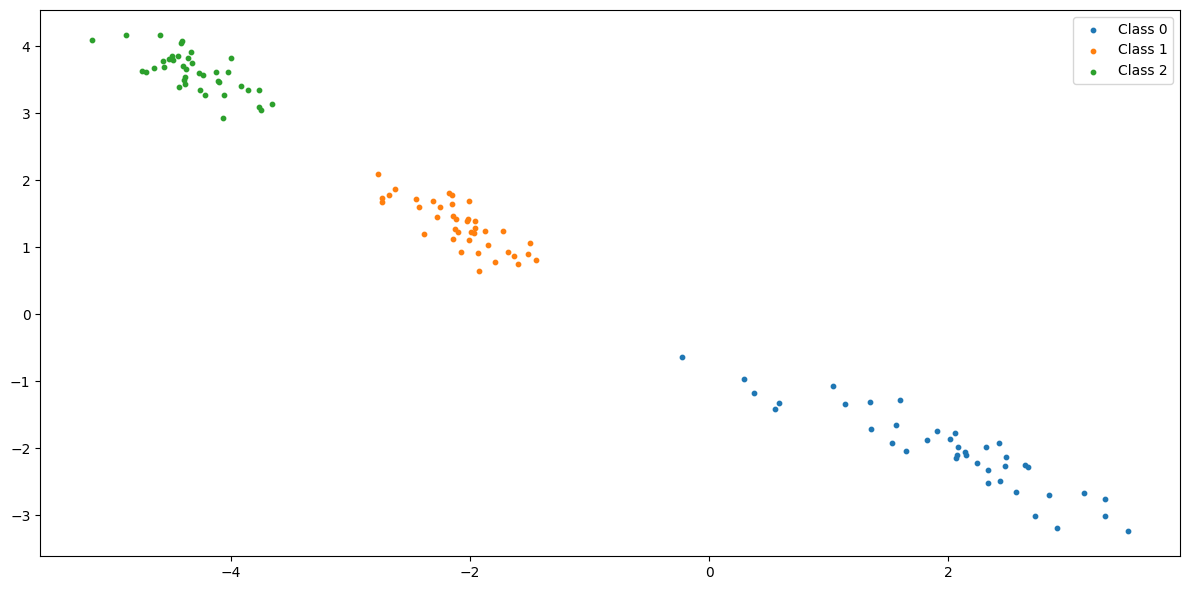
\includegraphics[width=0.8\textwidth]{images/reconstruction.png}
\caption{Graficación de la reconstrucción.}
\end{figure}


\subsection{Clasificador con Encoder Congelado}

Por último, se realizó un clasificador (Fully Connected + Softmax) que se entrenó congelando el \textit{encoder}. Para ello, se creó el modelo secuencial para la clasificación con una capa densa de activación Softmax que clasificase las 3 clases y se compiló con early stopping.
De este modo, tras entrenarlo con 150 épocas, terminó el entrenamiento con los siguientes resultados:

\begin{figure}[H]
\centering
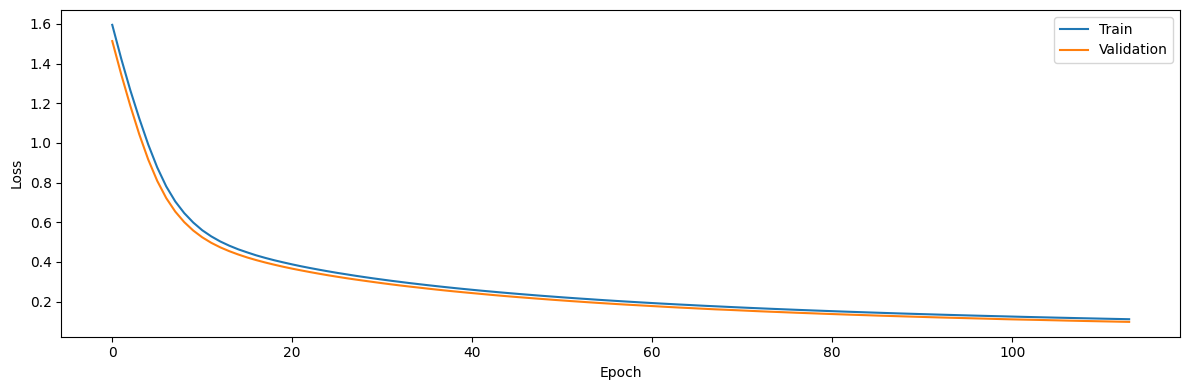
\includegraphics[width=0.8\textwidth]{images/accuracy_loss_frozenencoder.png}
\caption{Gráfica de la pérdida del modelo de clasificación.}
\end{figure}
\begin{figure}[H]
\centering
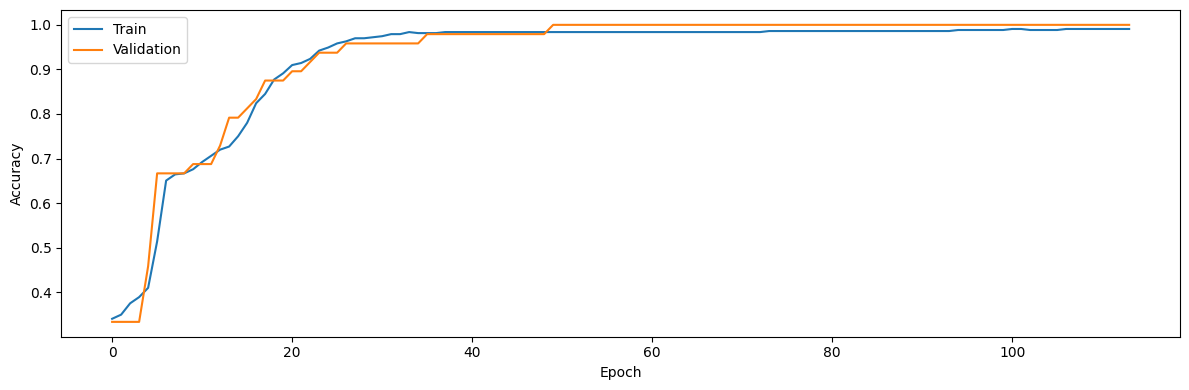
\includegraphics[width=0.8\textwidth]{images/accuracy_frozenencoder.png}
\caption{Gráfica de la precisión del modelo de clasificación.}
\end{figure}

\section{Resultados}

El modelo clasificador logró una precisión del 100 \% al predecir las etiquetas del conjunto de prueba. La siguiente gráfica muestra la proyección de las representaciones comprimidas en generadas por el encoder y la clasificación asignada por el modelo:

\begin{figure}[H]
\centering
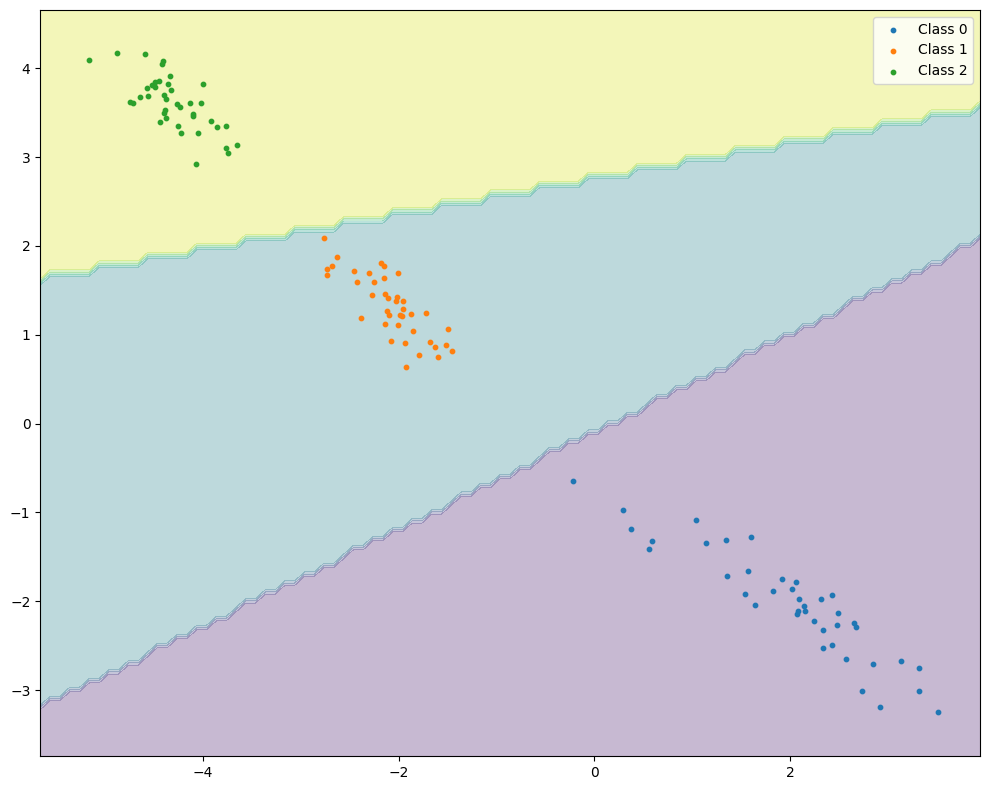
\includegraphics[width=0.8\textwidth]{images/decision_boundaries.png}
\caption{Representación de la clasificación del modelo.}
\end{figure}

Esto confirma la capacidad del pipeline completo para separar efectivamente las clases originales en un espacio reducido, preservando la estructura de los datos.





\section{Conclusión}

En esta práctica se implementaron diversas técnicas de reducción de dimensionalidad y clasificación, utilizando un conjunto de datos sintético generado en \(\mathbb{R}^{10}\). Estas técnicas incluyeron métodos tradicionales como Sammon Mapping, PCA, LDA y t-SNE, así como un enfoque basado en aprendizaje profundo mediante una red neuronal Encoder-Decoder.

Los resultados demostraron que las técnicas implementadas son efectivas para reducir la dimensionalidad del dataset, preservando la separación entre las clases en el espacio proyectado. En particular, el método t-SNE mostró su capacidad para identificar agrupamientos locales no lineales, mientras que LDA maximizó la separación entre clases usando información supervisada. Por otro lado, el Encoder-Decoder logró aprender representaciones comprimidas en \(\mathbb{R}^{2}\), que fueron utilizadas con éxito para clasificar las muestras con una precisión del 100 \% al congelar el encoder y añadir una cabeza de clasificación.

\newpage
\appendix
\section*{Apéndice}
El código relacionado con este documento está disponible en el siguiente enlace de GitHub:
\begin{center}
    \href{https://github.com/angelleon01/aprendizaje_profundo}{github.com/angelleon01/aprendizaje\_profundo}
\end{center}

\end{document}

